\section{Accuracy of current methods for predicting roll damping}
\label{se:accuracy_SI_method}
\parencite{kawahara_simple_2011} demonstrated that the Ikeda's method does not work for some modern ships with buttock flow stern. \parencite{soder_assessment_2019} also showed that the Ikeda's method was not capable to accurately predict the roll damping for a Pure Car and Truck Carrier. The SI-method being the simplified version of Ikeda's method most likely inherits its problems but also introduces some extrapolation errors as reported by \parencite{rudakovic_application_2017}. In the following, 227 existing roll decay model tests conducted at SSPA Maritime Dynamics Laboratory are used to validate the SI-method. The comparison will help to identify the drawbacks and improvement potentials of the SI-method. It aims at further developing this method to increase its accuracy based on the large test database through some statistical regression analysis.

\subsection{Overall accuracy of Ikeda\'s method}
\label{se:overall_comparison}
In the following, we will present an overall comparison between Ikeda\'s method and the damping estimated from experimental test database in order to identify possible potential to improve Ikeda\'s method.


Figure \ref{fig:B_e_hat_ikeda} shows a comparison of the nondimensional equivalent linear damping from model tests and the simplified method.  

\begin{figure}[H]
    \centering
    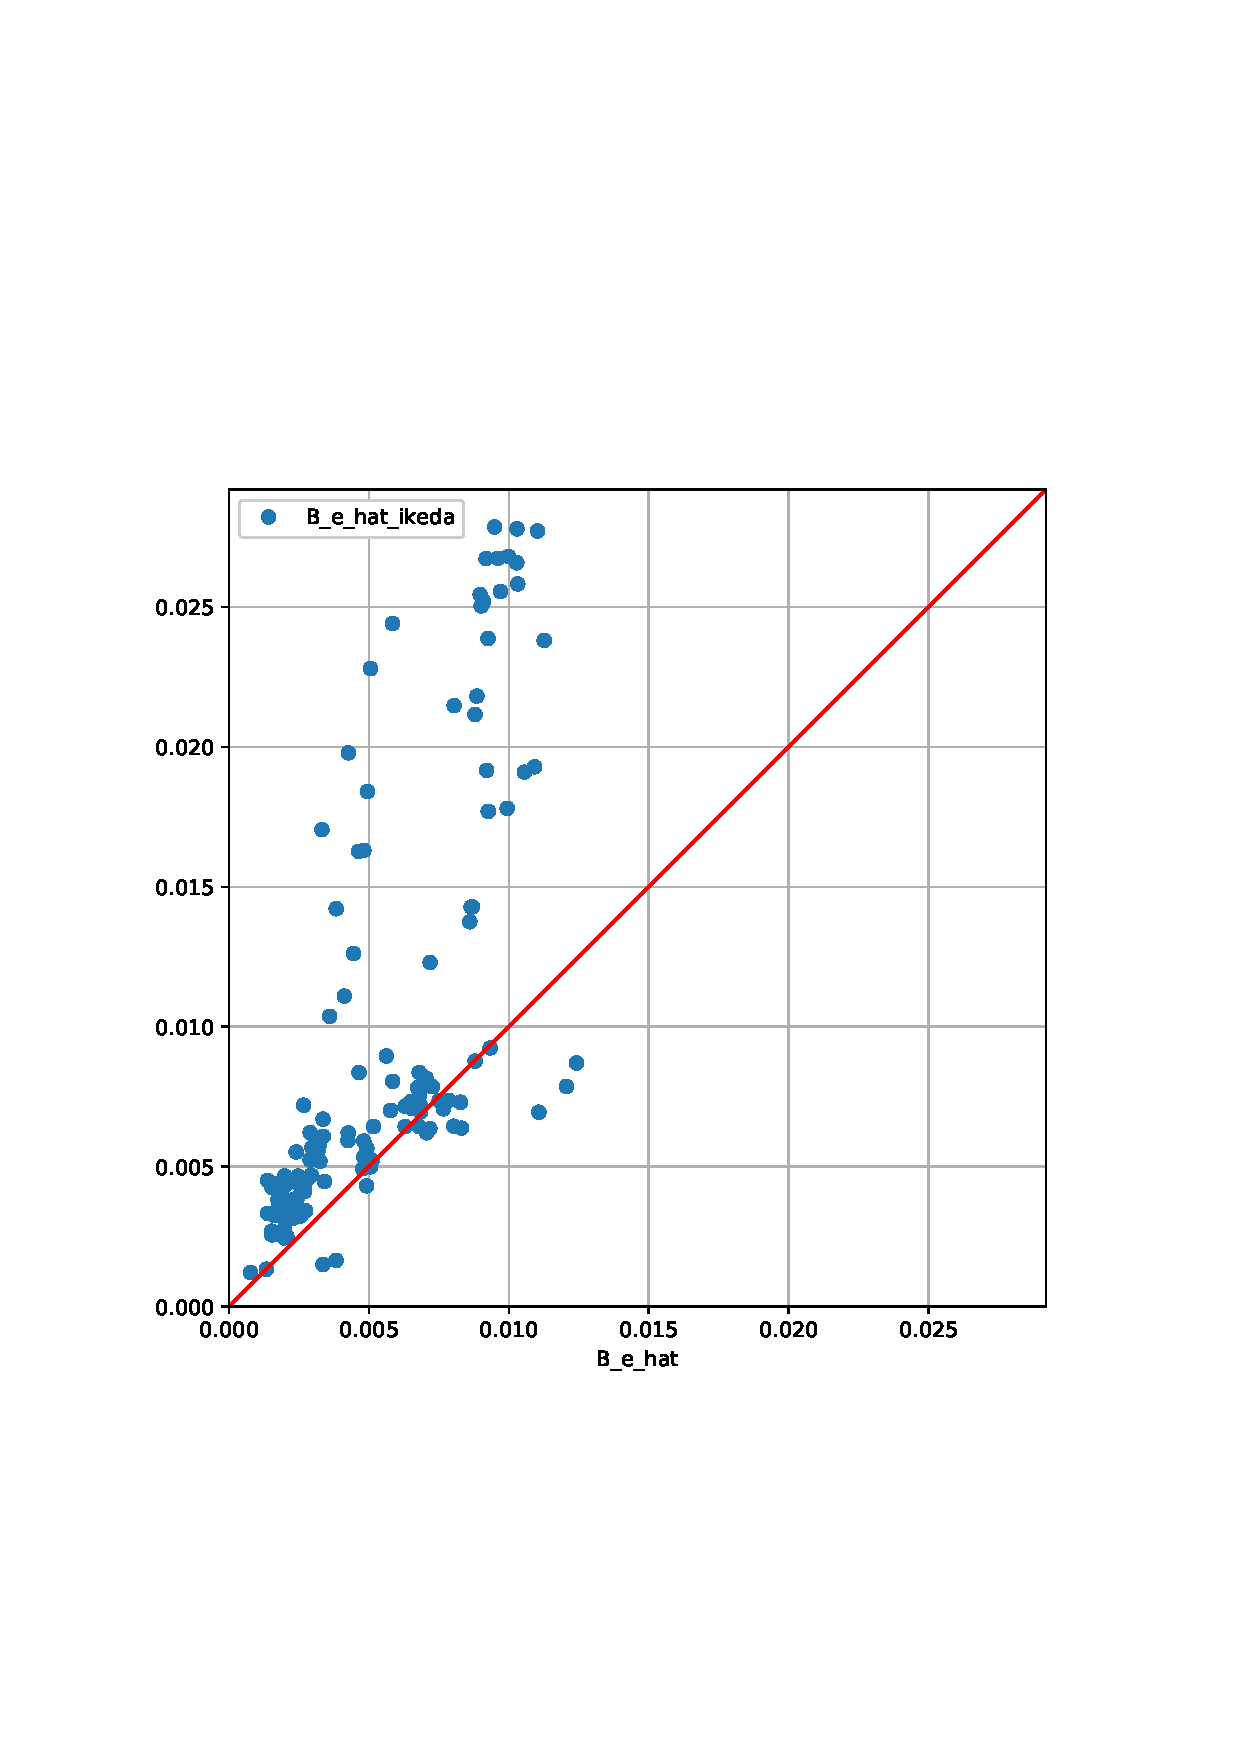
\includegraphics[width=\columnwidth]{figures/B_e_hat_ikeda.pdf}
    \caption{Nondimensional linearized damping from model tests and simplified Ikeda}
    \label{fig:B_e_hat_ikeda}
\end{figure}

When plotting the error between the model test and simplified Ikeda method in figure \ref{fig:B_e_hat_error} this shows that the error is much larger for $T/L_{pp}<0.034$

\begin{figure}[H]
    \centering
    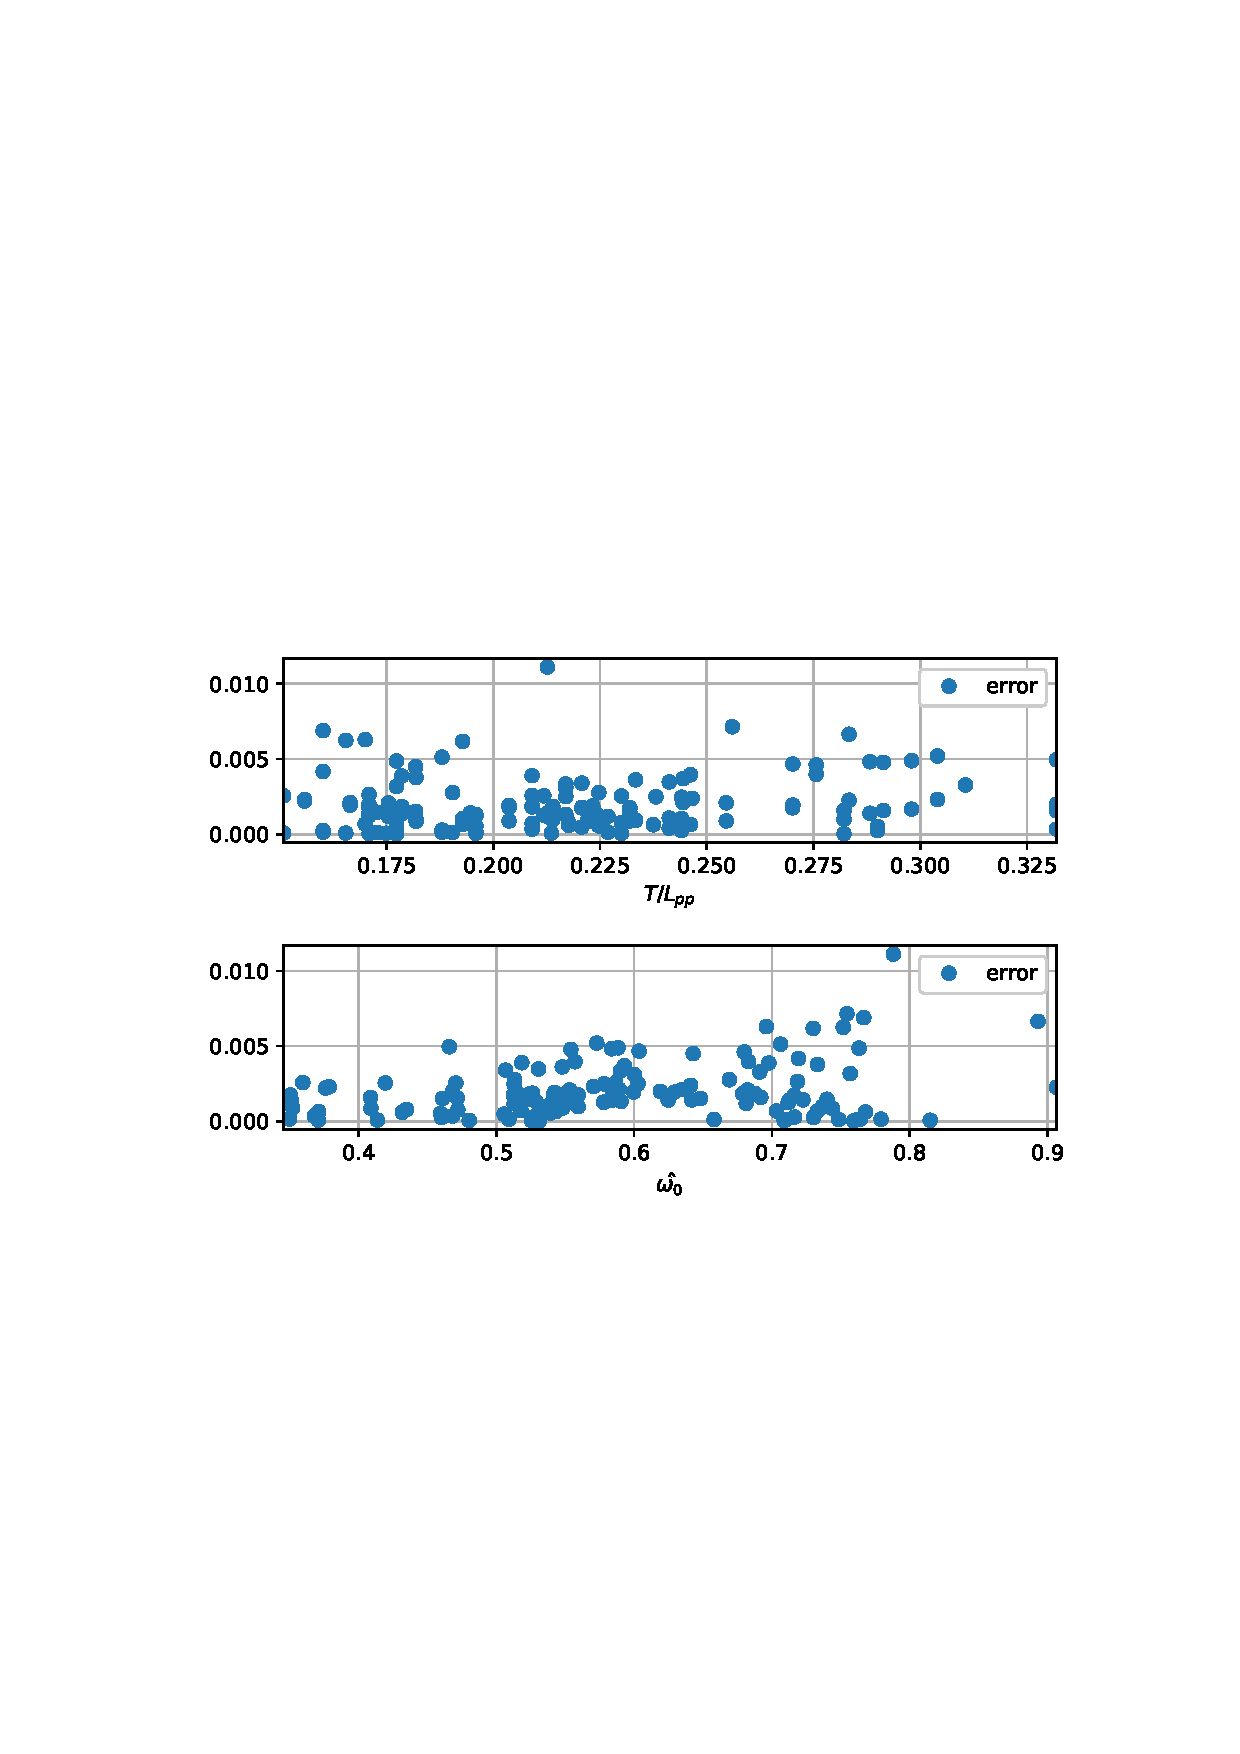
\includegraphics[width=\columnwidth]{figures/B_e_hat_error.pdf}
    \caption{Simplified Ikeda error versus draught}
    \label{fig:B_e_hat_error}
\end{figure}

Figure \ref{fig:B_e_hat_good} shows the comparison for only model tests with $T/L_{pp}>0.034$.
This confirms the small draft to beam ratio limit of this method as mentioned in \cite{kawahara_simple_2011}. The corresponding $R^2$ score is 0.38.

\begin{figure}[H]
    \centering
    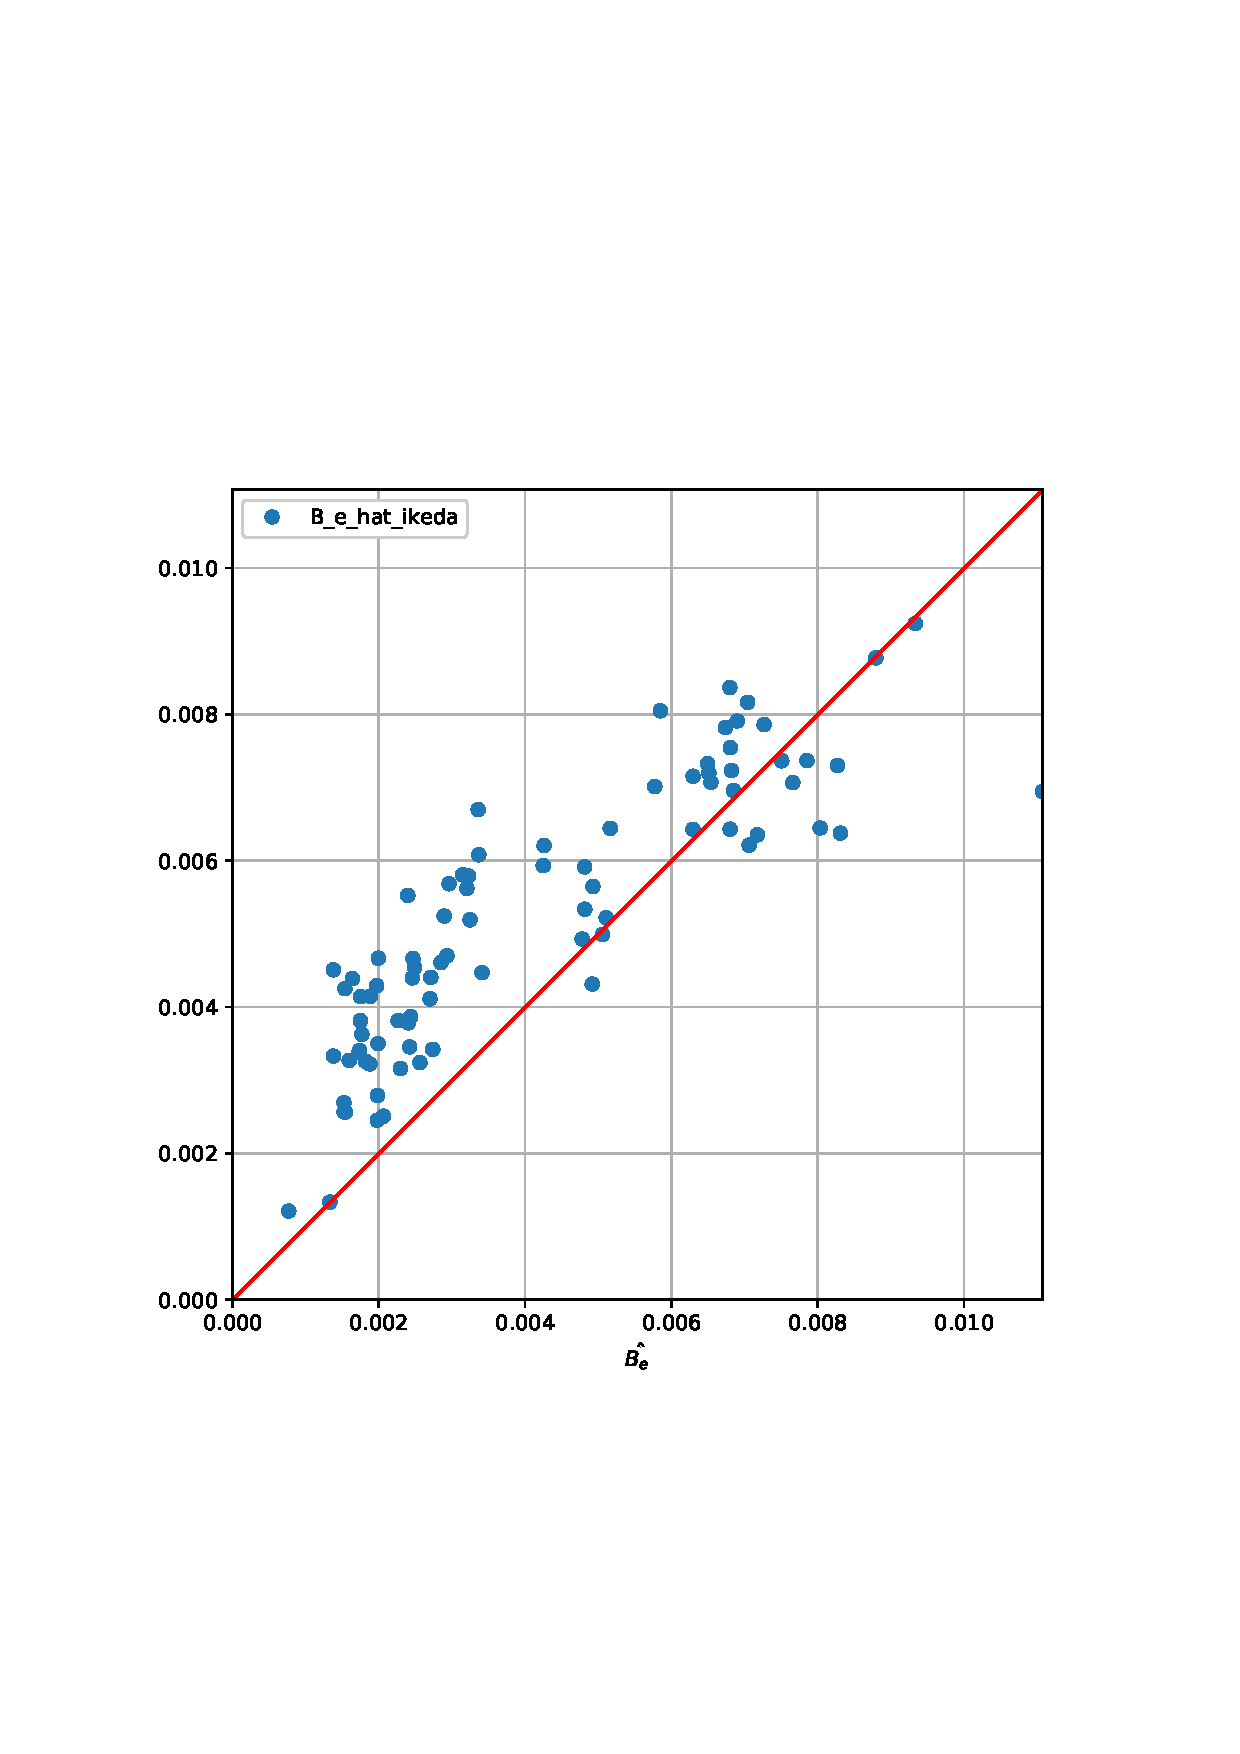
\includegraphics[width=\columnwidth]{figures/B_e_hat_good.pdf}
    \caption{Nondimensional linearized damping from model tests and simplified Ikeda $T/L_{pp}>0.034$}
    \label{fig:B_e_hat_good}
\end{figure}


\subsection{Sensitivity analysis of the SI-method for all database ships}
\label{se:accuracy_SI_method}
Since a very large discrepancy between the model test results and the SI-method was observed for both the limited and unlimited approach, a sensitivity study of the SI-method was carried out. A so-called ``reference ship" with ship parameters located in the middle of the SI-method applicable boundaries as in Eq. (\ref{eq:SI_limits}) is used for the investigation. For the sensitive study, only the relatively important ship parameters, i.e., $C_b$,$\frac{Beam}{T}$, $\frac{\overline{OG}}{T}$, $A_0$, $\frac{BK_B}{Beam}$, $\frac{BK_L}{L_{pp}}$, are chosen to investigate the effects of their variation on different roll damping components.

The results of the sensitivity analysis are presented in Fig. \ref{fig:SI_sensitivity}. It can be seen that the wave damping component $B_W$ increases a lot with the absolute value of $\overline{OG}/T$. It can be also seen that the wave damping has an enormous increase when the beam to draught ratio exceeds the input boundary, which seems to be the case for at least one third of the roll decay tests. It can also be noted that most of the ships in the database have midsection coefficients $A_0$ and bilge keel heights outside the limits. The unrealistic prediction of wave damping component $B_W$ in terms of $\frac{Beam}{T}$ and $\frac{\overline{OG}}{T}$ should be further examined. The big variation might be caused by the improper ship parameter $\frac{Beam}{T}$ that is outside the boundaries used in the SI-method. In the following the SI-method is further examined by comparing it to corresponding results with the original Ikeda's method.

\begin{figure}[H]
    \centering
    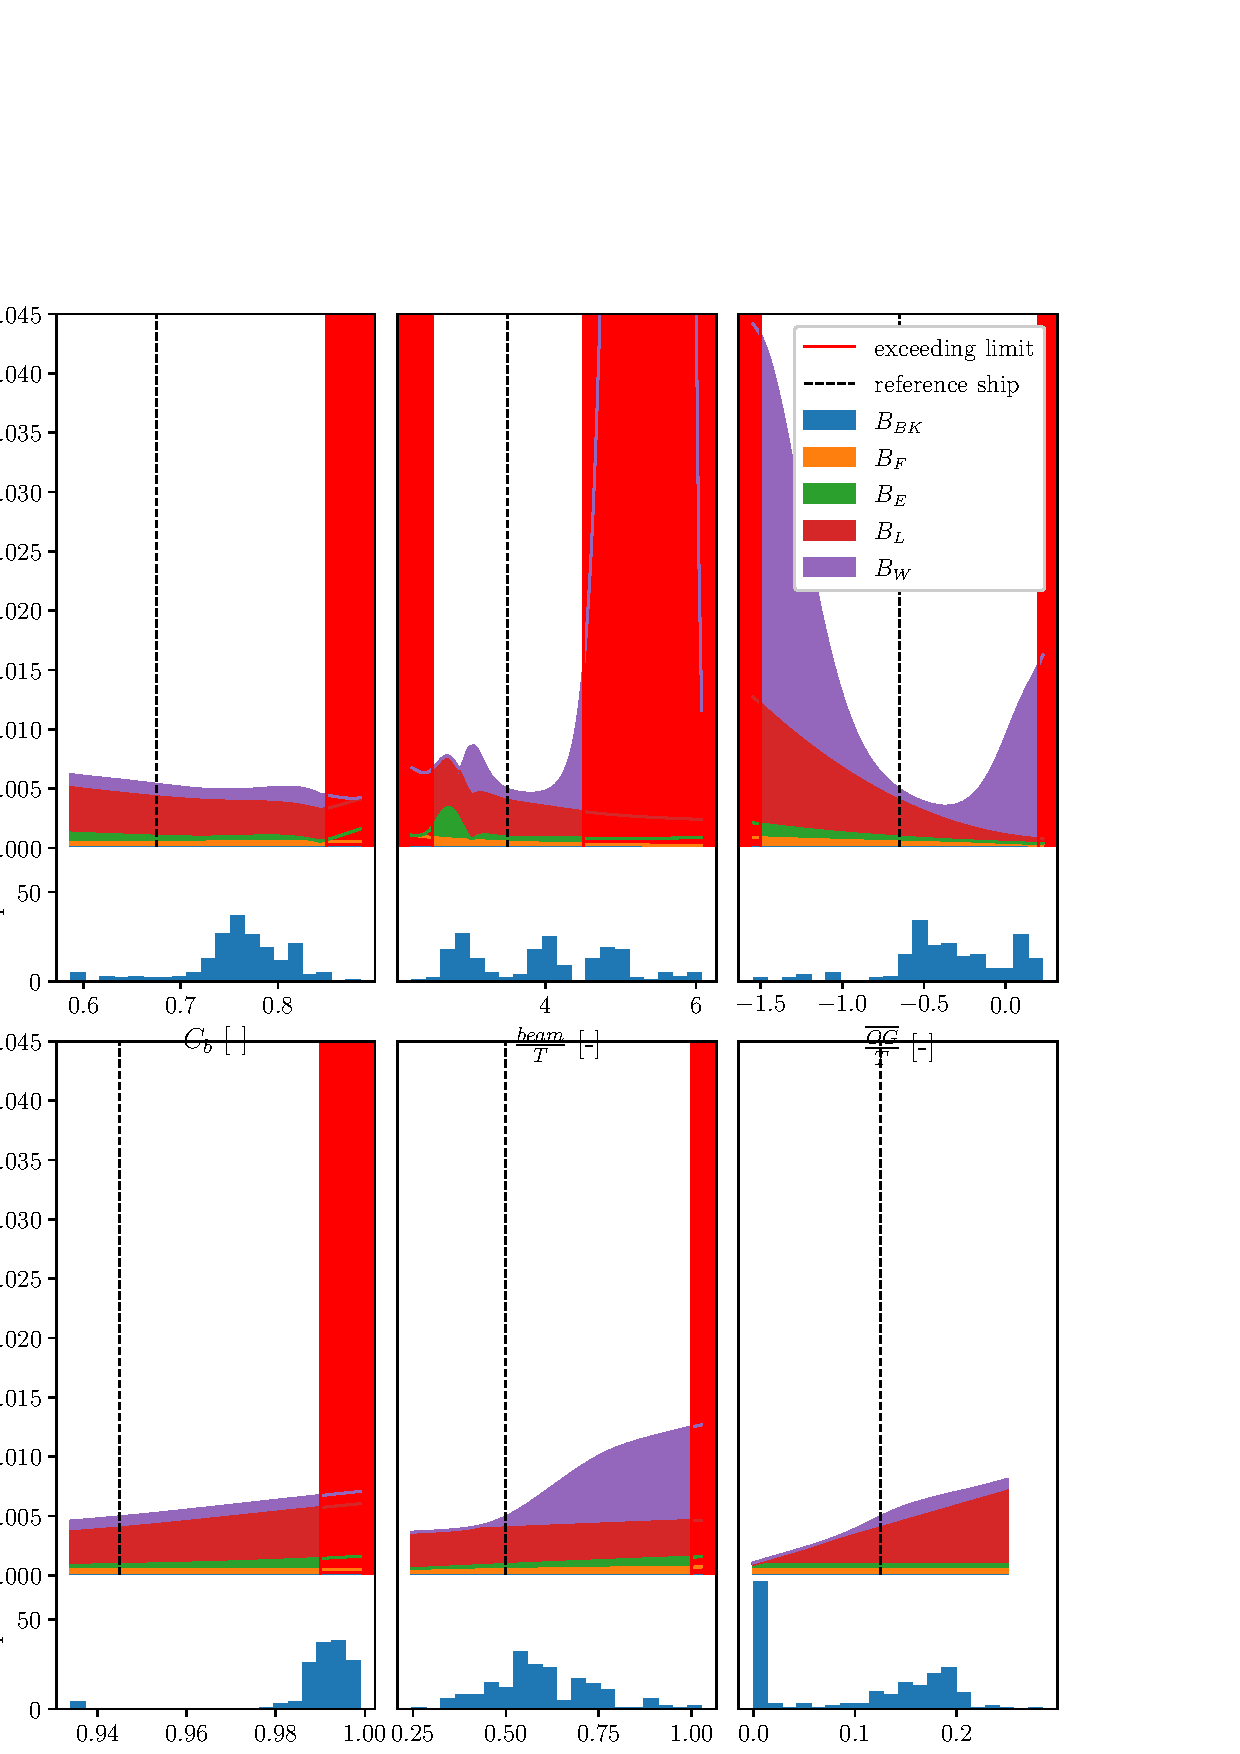
\includegraphics[width=0.95\textwidth]{figures/SI-sensitivity.pdf}
        \vspace{-0.1cm}
    \caption{SI-method input parameter variation and data base ships}
    \label{fig:SI_sensitivity}
\end{figure}


\subsection{Simplified and original Ikeda method}
\label{se:si_ikeda_model}
Comparing the results from the SI-method from corresponding results with the original Ikeda's method can be a way to see whether the observed deviations are result from extrapolation or inherent in the original method. In Ikeda's method, more detailed information about the ship hull geometry is needed so that $B_W$ can be calculated with a strip method and $B_E$ can be calculated using sectional Lewis coefficients. It was possible to collect the required hull inputs for 15 ships in the database. These ships were used in 50 of the reference roll decay tests: all but one of the tests exceed the limits. Ikeda's method has a much better agreement for these exceeding model tests according to Fig.\ref{fig:si_ikeda_model} and the calculated $R^2$ in Table \ref{tab:si_ikeda_validation}.

\begin{figure}[H]

    \centering
    \includegraphics[width=0.4\textwidth]{figures/si_ikeda_model.eps}
    \caption{Comparison of SI, Ikeda and model tests}
    \label{fig:si_ikeda_model}

\end{figure}

\input{equations/si_ikeda_validation}

